\chapter{SKY130 Interface with eSim}
\label{chap9}
\thispagestyle{empty}

SkyWater Open Source PDK provides a completely open source Process Design Kit for the 130nm Technology Node. SKY130 PDK provides a lot many features and components to its library. The MPW Shuttle is a free chip fabrication shuttle program sponsored by the Google where the designs made using the SKY130 PDK may be fabricated at no cost.

eSim being an Open Source EDA Tool has being interfaced with the SKY130 PDK. eSim-2.3 and above is supporting the PDK. Currently only the primitive libraries(sky130\_fd\_pr) are supported, however, the symbols for other libraries are also loaded in eSim, so even the other ones can be interfaced with eSim with few manual changes.

The various steps involved in simulating a circuit schematic in eSim interfaced with SKY130 are explained in the sections below:
\section {Schematic Creation}
\begin{itemize}

\item The steps of opening the Eeschema and editing are same as mentioned in the previous Chapters.
\item To create a Schematic in eSim for SKY130, one needs to use the SKY130 components.
\item The SKY130 components are available in the \textbf{eSim\_SKY130} library. It can be chosen by clicking on the \textbf{Place Component} button on the Right Toolbar and searching for the same in the \textbf{Choose Component} Dialog Box.

\begin{figure}[H]
\centering
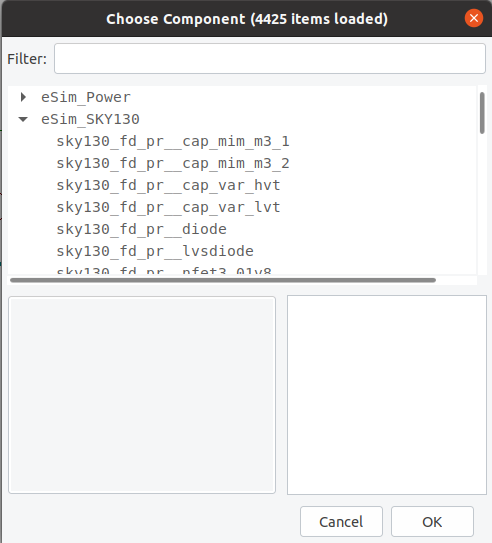
\includegraphics[ height = 5cm]{./SKY130/SKY130libraries.png}
\caption{eSim\_SKY130 Libraries}
\label{eSimSKY130 Libraries}
\end{figure}
\item One may even chose the predefined IPs made in SKY130 available in eSim. These IPs are available in the \textbf{eSim\_SKY130\_Subckts} library. It can be chosen by clicking on the \textbf{Place Component} button on the right Toolbar and searching for the same.

\begin{figure}[H]
\centering
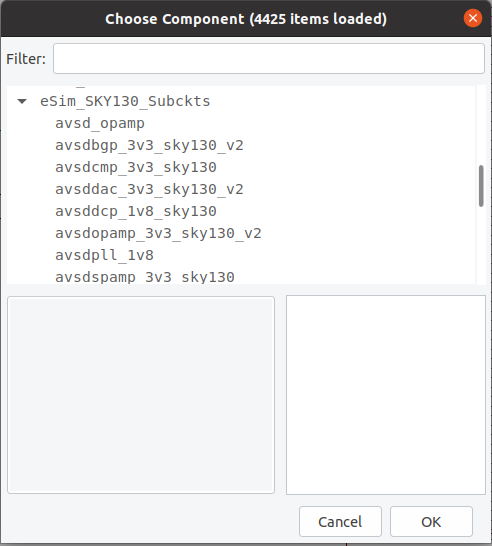
\includegraphics[ height = 5cm]{./SKY130/SKY130subcktlibraries.png}
\caption{eSim\_SKY130\_Subckts IP Libraries}
\label{eSimSKY130Subckts IP Libraries}
\end{figure}
\item \textbf{It is important to choose the SKY130mode from the eSim\_SKY130 to switch eSim into the SKY130 mode.}
\begin{figure}[H]
\centering
\includegraphics[ height = 5cm]{./SKY130/SKY130Mode.png}
\caption{SKY130Mode}
\label{SKY130Mode}
\end{figure}
\item Let us look into the CMOS Inverter as an example. Here is an example schematic of a CMOS Inverter made from the SKY130 components:
\begin{figure}[H]
\centering
\includegraphics[ height = 8cm]{./SKY130/SKY130InverterSchematic.png}
\caption{CMOS Inverter Schematic using SKY130 components}
\label{eSimSKY130Subckts IP Libraries}
\end{figure}
\item Note: While using SKY130mode in eSim, use the components of designators `sc', `u', `x', `v', `i', `a'. This is to ensure that other necessary technology node does not get included while in the SKY130 mode.
\item Annotate the schematic and generate the netlist. Please follow the steps given in previous chapters to do the same.

\end{itemize}

 \section {KiCad to Ngspice Conversion}

\begin{itemize}
\item Click on the \textbf{Convert KiCad to Ngspice Button} available in the Left Toolbar of the eSim Main Window.
\item Add all the simulation parameters and the Source details in the \textbf{Analysis Tab} and the \textbf{Source Details Tab}. Refer previous chapters of this manual to do the same.
\item Click on the \textbf{Device Modeling Tab}.
\item The options for the SKY130 PDK are involved in the \textbf{Device Model Tab}. The Device Model Tab for the CMOS Inverter project is shown in Fig. \ref{DeviceModelTab}.
\begin{figure}[H]
\centering
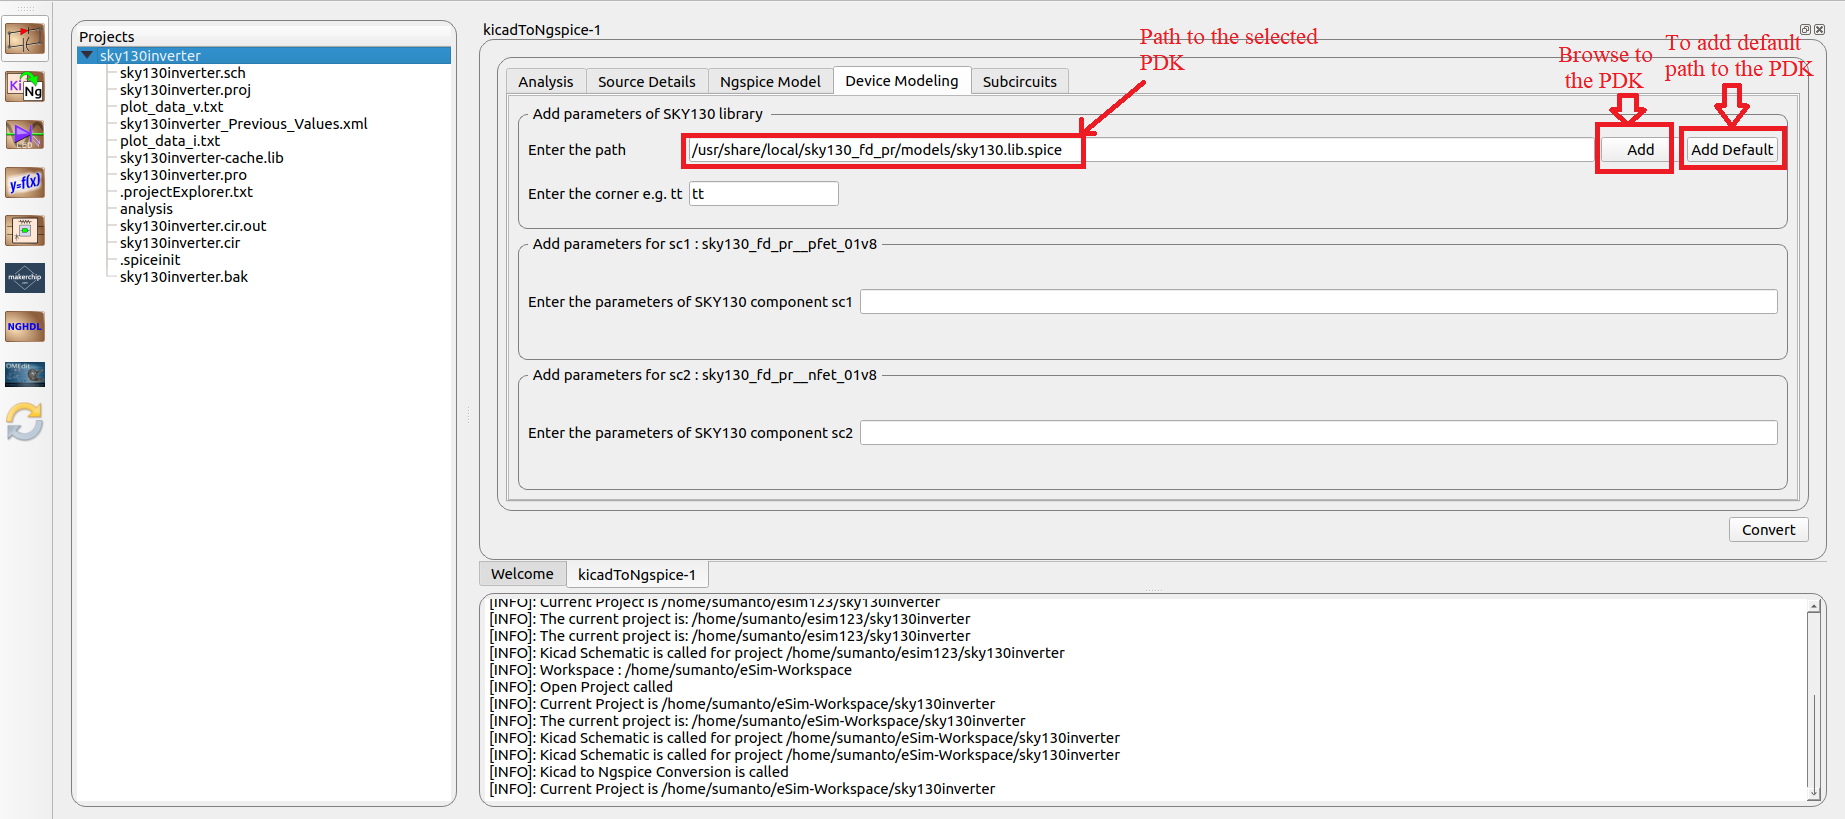
\includegraphics[ height = 5cm]{./SKY130/DeviceModelTab.png}
\caption{Device Model Tab of CMOS Inverter using SKY130}
\label{DeviceModelTab}
\end{figure}
\item The user may select the \textbf{Add Default Path} option to add the Default Path of the PDK installed along with eSim. Note that only primitive libraries(sky130\_fd\_pr) are present here.
\item In order to select path to any other SKY130 PDK, the user may add the path by clicking on the \textbf{Add} button.
\item The user can add the SPICE model parameters for the components in the text-box provided.
\item If a SKY130 Subcircuit IP is added in the  circuit. Then Click on the \textbf{Subcircuits Tab}. For Example, refer Fig.\ref{Subcircuits Tab}.
\begin{figure}[H]
\centering
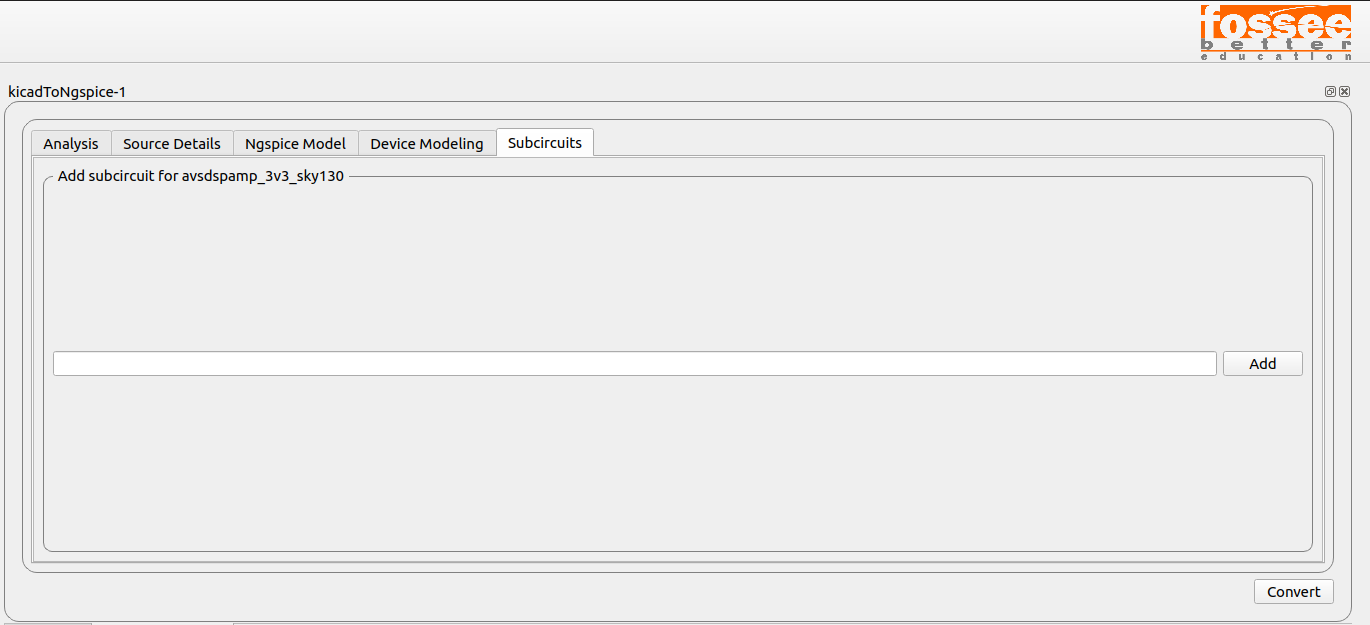
\includegraphics[ height = 7cm]{./SKY130/Subcircuits.png}
\caption{Subcircuits Tab}
\label{Subcircuits Tab}
\end{figure}
\item Click on the \textbf{Add} button.
\item Browse to the SKY130 folder and Click on it. Click the IP Subcircuit to be included. Click on the Open Button on the top right corner.
\begin{figure}[H]
\centering
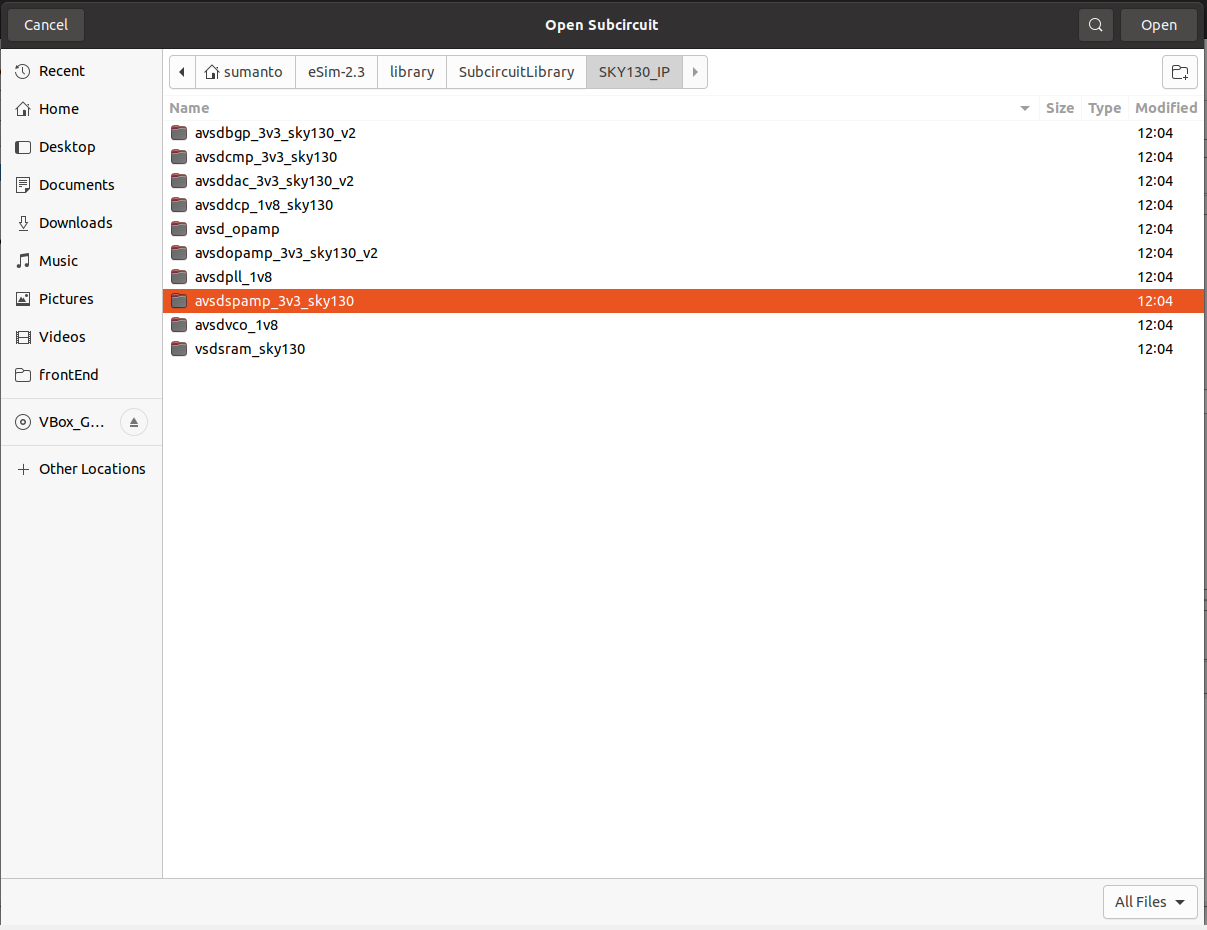
\includegraphics[ height = 6cm]{./SKY130/SubcircuitsPath.png}
\caption{Adding path to the Subcircuit}
\label{SubcircuitsPath}
\end{figure}
\item The Subcircuit chosen gets added. Refer Fig. \ref{SubcircuitsAdded}.
\begin{figure}[H]
\centering
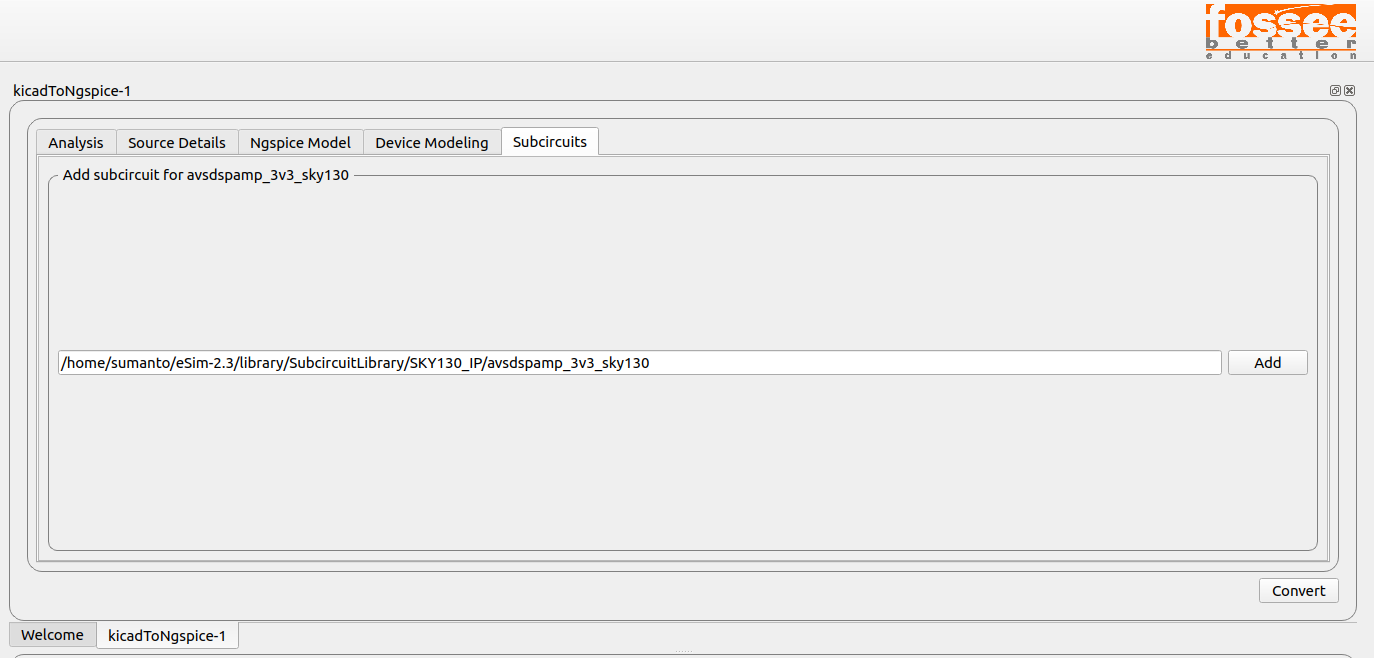
\includegraphics[ height = 6cm]{./SKY130/Subcircuitsadded.png}
\caption{Subcircuit Added}
\label{SubcircuitsAdded}
\end{figure}
\item Click on the \textbf{Convert} button.
\item A Dialog Box \textbf{The KiCad to Ngspice conversion completed successfully!} appears on the screen showing that the conversion is successful.
\item If something needs to be added manually, Click on the \textbf{ \textit{Project\_Name}.cir.out} file in the left \textbf{Project Panel} and the file can be edited manually. Refer Fig. \ref{netlist} as an example.
\begin{figure}[H]
\centering
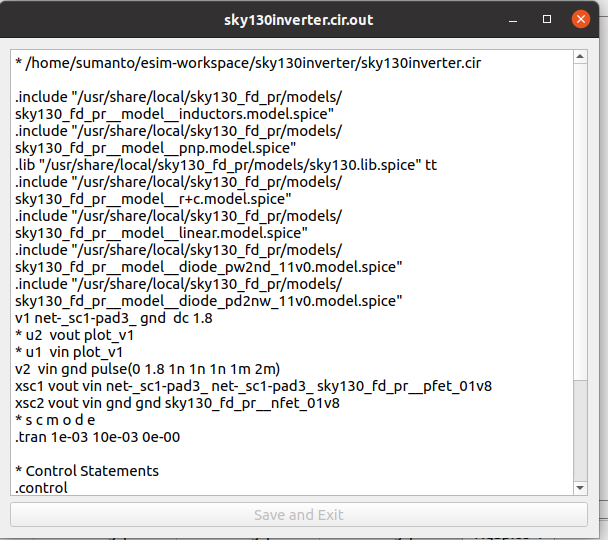
\includegraphics[ height = 6cm]{./SKY130/netlist.png}
\caption{Manually Editing the Netlist}
\label{netlist}
\end{figure}
\end{itemize}

\section {Run Simulation}
\begin{itemize}
\item To run the simulation, Click on the \textbf{Simulate} button on the Left Toolbar.
\item Refer Fig. \ref{Simulation Results} for the simulation results of the CMOS Inverter using SKY130.
\begin{figure}[H]
\centering
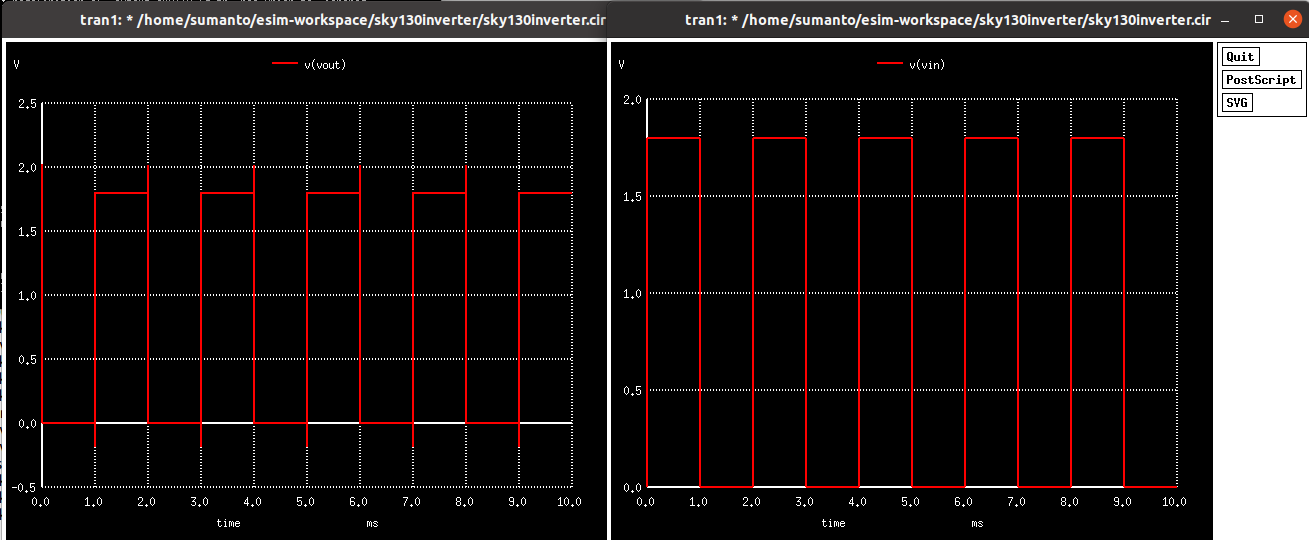
\includegraphics[ height = 6cm]{./SKY130/Simulation.png}
\caption{Simulation Results of CMOS Inverter using SKY130}
\label{Simulation Results}
\end{figure}
\end{itemize}
In this way, the SKY130 PDK has been interfaced with eSim.
